\documentclass[8pt]{extarticle}
\usepackage{graphicx,blindtext,amsthm,tikz,wrapfig,amssymb,amsmath,xcolor,siunitx,breqn,caption,cancel,esdiff,multicol,multicol,xparse,stmaryrd,hyperref} % Required for inserting images
\usepackage[a4paper,top=0.5cm, bottom=0.5cm, left=0.5cm, right=0.5cm]{geometry}
\usetikzlibrary{positioning, arrows.meta}

\setlength{\columnsep}{0.2cm}


\DeclareMathOperator{\di}{\;d\!}
\DeclareMathOperator{\sech}{sech}
\DeclareMathOperator{\cosech}{csch}
\DeclareMathOperator{\arsec}{arsec}
\DeclareMathOperator{\arcot}{arCot}
\DeclareMathOperator{\arcosech}{arCsc}
\DeclareMathOperator{\arcosh}{arCosh}
\DeclareMathOperator{\arsinh}{arsinh}
\DeclareMathOperator{\artanh}{artanh}
\DeclareMathOperator{\arsech}{arsech}
\DeclareMathOperator{\arcsch}{arCsch}
\DeclareMathOperator{\arcoth}{arCoth}

\setlength{\parindent}{0pt}
\setlength{\abovedisplayskip}{1pt}
\setlength{\belowdisplayskip}{1pt}
\setlength{\abovedisplayshortskip}{0pt}
\setlength{\belowdisplayshortskip}{1pt}
\setlength{\jot}{1pt}

\newsavebox{\fitdisplaybox}
\newcommand{\fitdisplay}[1]{%
  \par\vspace{-1pt}\noindent
  \sbox{\fitdisplaybox}{#1}%
  \makebox[\columnwidth][c]{%
    \ifdim\wd\fitdisplaybox>\columnwidth
      \resizebox{\columnwidth}{!}{#1}%
    \else
      \usebox{\fitdisplaybox}%
    \fi
  }%
  \par\vspace{-1pt}%
}

% ===== Custom theorem-like environments with decimal numbers =====
% Paste this whole block into your preamble.

\newcounter{customthm}   % internal counter for cross‑referencing
\makeatletter

% Helper: define a theorem-like environment.
% #1 = environment name (e.g. theorem)
% #2 = printed heading (e.g. Theorem)
% #3 = style: plain, definition, remark
\newcommand{\definetheorem}[3]{%
  \newenvironment{#1}[1]{%
    \refstepcounter{customthm}%           % unique internal label
    \renewcommand{\@currentlabel}{##1}%   % store the custom decimal number
    \par\noindent
    \ifx#3plain\relax
      \textbf{#2 ##1.}\ \itshape
    \else\ifx#3definition\relax
      \textbf{#2 ##1.}\ \normalfont
    \else\ifx#3remark\relax
      \textit{#2 ##1.}\ \normalfont
    \else
      \textbf{#2 ##1.}\ \normalfont
    \fi\fi\fi
    \ignorespaces
  }{%
    \par
  }%
}

\makeatother

% Now create the environments you asked for.
\definetheorem{theorem}{Theorem}{plain}
\definetheorem{lemma}{Lemma}{plain}
\definetheorem{proposition}{Proposition}{plain}
\definetheorem{corollary}{Corollary}{plain}
\definetheorem{definition}{Definition}{definition}
\definetheorem{remark}{Remark}{remark}

\newenvironment{example}{%
  \par\noindent
  \textbf{Example.}\ \normalfont
  \ignorespaces
}{%
  \par
}

\makeatletter
\renewenvironment{proof}[1][\proofname]{%
  \par%
  \pushQED{\qed}%
  \normalfont
  \topsep=2pt\partopsep=0pt\parsep=0pt\itemsep=0pt%
  \trivlist
  \item[\hskip\labelsep\itshape #1\@addpunct{.}]\ignorespaces
}{%
  \popQED\endtrivlist\@endpefalse
  \vspace{-1pt}%
}
\makeatother

\begin{document}
\fontsize{6}{7}\selectfont

    \begin{multicols}{5}
    \raggedright

        {\centering\fontsize{7.8}{8.5}\selectfont\textbf{Proofs}\par}
        \vspace{2pt}
        
        \begin{theorem}{1.1}
            (The Division Theorem for \(\mathbb{Z}\)): \(a,b\in\mathbb{Z}\) with \(b>0\) \(\exists ! q,r\in\mathbb{Z}\) with \(0\le r<b\) s.t. \(a=bq+r\).
        \end{theorem}

        \begin{proof}
            (\textit{Existance}):
            Let \(R=\{a-bm:m\in\mathbb{Z} \;\&\; a-bm\ge0\}\),
            then as:
            if \(a\ge0\), \(a-b\cdot 0=a\ge0\) so \(a\in R\);
            if \(a<0\), \(a-b\cdot a=a(1-b)\ge0\) so \(a-b\cdot a\in R\),
            \(R\ne\varnothing\).
            Thus, take \(r=\min(R)\) \& so \(0\le r=a-bm\in R\) for some \(m\in\mathbb{Z}\),
            choose \(q=m\in\mathbb{Z}\).
            So by construction \(a=bq+r\).
            Note, \(r<b\) as were such not true then \(r>a-b(q+1)=r-b\in R\) but this contradicts \(r=\min(R)\), so we have \(0\le r<b\).
            (\textit{Uniqueness}):
            Suppose \(q,q',r,r'\in\mathbb{Z}\) with \(0\le r',r<b\) \& \(a=bq+r=bq'+r'\),
            also WLOG take \(r'\le r\).
            So with \(\frac{r-r'}b\in(-1,1)\), \& \(\frac{r-r'}b=\frac{a-bq-(a-bq')}b=q'-q\in\mathbb{Z}\),
            we have \(\frac{r-r'}b=0\) i.e. \(r=r'\).
            So \(q=\frac{a-r}b=\frac{a-r'}b=q'\).
        \end{proof}

        \textbf{Euclidian Algorithm:}

        Let \(a,b\in\mathbb{Z}^+\), apply Th\textsuperscript{m} 1.1, to give:

        \fitdisplay{\(\begin{aligned}
            a&=bq_1+r_1\\
            b&=r_1q_2+r_2\\
            r_1&=r_2q_3+r_3\\
            &\hspace{5pt}\vdots\\
            r_{n-1}&=r_nq_{n+1}\text{,}
        \end{aligned}\)}

        Here, \(\gcd(a,b)=r_n\).
        To prove this relation \(G(r_{i},r_{i+1})=G(r_{i+1},r_{i+2})\), where \(G(a,b)=\{n\in\mathbb{Z}:n|a\;\&\;n|b\}\).

        \textbf{Reverse Euclid:}

        Given a completed algorithm we can obtain \(n,m\in\mathbb{Z}\) s.t. \(na+mb=\gcd(a,b)\) i.e. taking the end of a Euclidian algroithm:

        \fitdisplay{\(\begin{aligned}
            &\hspace{5pt}\vdots\\
            r_{n-3}&=r_{n-2}q_{n-1}+r_{n-1}\quad(1)\\
            r_{n-2}&=r_{n-1}q_{n}+r_{n}\quad(2)\\
            r_{n-1}&=r_{n}q_{n+1}
        \end{aligned}\)}

        we have:

        \fitdisplay{\(\begin{aligned}
            \text{(2)}\Rightarrow r_n&=r_{n-2}-r_{n-1}q_n\quad(3)\\
            \text{(1)}\Rightarrow r_{n-1}&=r_{n-3}-r_{n-2}q_{n-1}\quad(4)\\
            \text{(3) \& (4)}\Rightarrow r_n&=r_{n-2}-(r_{n-3}-r_{n-2}q_{n-1})q_n\\
            &\hspace{5pt}\vdots
        \end{aligned}\)}

        we continue this ladder up, simplifying each time,
        {\footnotesize (Note: \(r_{n}=\gcd(a,b)\))}

        \begin{theorem}{1.9}
            Every integer \(n\ge2\) can be written as a product of primes.
        \end{theorem}

        \begin{proof}
            (\textit{By strong induction}):

            (\textit{Base case}, \(n=2\)): Trivially true, \(n=2\) a product of primes.

            (\textit{Inductive Hypothesis}): Suppose for \(n\in{2,3,\ldots,k}\) \(n=p_{n,1}p_{n,2}\cdots p_{n,m_n}\).
            
            Then for \(n=k+1\), if \(k+1\) is prime we are done, if not then \(k+1=ab\) where \(a,b\in\{2,3,\ldots,k\}\), thus \(a=p_{a,1}p_{a,2}\cdots p_{a,m_a}\) \& \(b=p_{b,1}p_{b,2}\cdots p_{b,m_b}\) so: \(k+1=p_{a,1}p_{a,2}\cdots p_{a,m_a}p_{b,1}p_{b,2}\cdots p_{b,m_b}\).

            So \(\forall n\in\mathbb{N}\) with \(n\ge2\), we are done.

        \end{proof}

        \begin{theorem}{1.10}
            (Euclid's property of primes) \(\forall p\in \text{Primes}\) \& \(\forall a,b\in\mathbb{Z}\). \(p|ab\implies p|a\text{ or } p|b\).
        \end{theorem}

        \begin{proof}
            (\textit{Case \(p|a\)}): We are done.

            (\textit{Case \(p\nmid a\)}): Then using the Euclidian algorithm we obtain: \(1=na-mp\) with \(n,m\in\mathbb{Z}\).
            So \(p|b\Longleftrightarrow p|(na-mp)b\Longleftrightarrow p|n(ab)-mbp\impliedby p|ab\).
        \end{proof}

        {\footnotesize the chain of implications uses a proposition in the notes which states: \(p|a\;\&\;p|b\implies p|a+b\;\&\;p|ab\)}.

        \begin{theorem}{1.12}
            (Fundamental Theorem of Arithmetic) \(\forall n\in\mathbb{N}\) with \(n\ge2\), \(\exists! p_1,p_2,\ldots,p_r\in\text{Primes}\) up to ordering, s.t.: \(n=p_1p_2\cdots p_r\).
        \end{theorem}

        \begin{proof}
            The existance is from Th\textsuperscript{m} 1.9. For uniqueness, suppose \(p_1p_2\cdots p_r=q_1q_2\cdots q_s\), then cancel common primes, suppose the result is not \(1\) i.e. we are left with \(p_1p_2\cdots p_n=q_1q_2\cdots q_m\) with \(p_i\ne q_j\),\(\forall i\in\{1,\ldots,n\}\) \& \(\forall j\in\{1,\ldots,m\}\), after reindexing. Then \(p_1|q_1q_2\cdots q_m\) so \(\exists j\in\{1,\ldots,m\}\)\(p_1|q_j\), but \(q_j\) is prime so \(p_1=q_j\), \(\lightning\).
        \end{proof}

        \begin{lemma}{1.16}
            \(\forall a,b\in R\): \(0a=a0=0\); \(a(-b)=(-a)b=-(ab)\); \& \((-a)(-b)=ab\)
        \end{lemma}

        \begin{proof}
            \(0a+0=0a=(0+0)a=0a+0a\) so \(0a=0\).
            
            \(ab+a(-b)=a(b-b)=a0=0=(a-a)b=ab+(-a)b\) so by the Groups \& Geo\textsuperscript{m} we have \(-(ab)\) is the unique element s.t. \(ab-(ab)=0\), \(a(-b)=-(ab)=(-a)b\).

            \((-a)(-b)=-(a(-b))=-(-(ab))=ab\).
        \end{proof}

        \begin{lemma}{1.18}
            (Subring Test) Let \(R\) be a ring \& \(S\subseteq R\). Then \(S\) is a subring of \(R\) iff the following hold, \(\forall r,s\in S\):

            \vspace{-10pt}
            \begin{enumerate}
                \item \(1_R\in S\),
                \vspace{-10pt}
                \item \(r+s,rs\in S\), \& 
                \vspace{-10pt}
                \item \(-r\in S\).
            \end{enumerate}
            \vspace{-10pt}
        \end{lemma}

        \begin{proof}
            By 1 \& 3 we have \(-1_R\in S\) so \(0_R=1_R-1_R\in S\) by 2. So \((S,+)\) is a group by the subgroup test with \((R,+)\).
            Commutativity of \(+\), associativity of \(+\) \& \(\times\), \& distributivity of \(\times\) over \(+\) are all inheritited from \(R\).
            Note, as they shair operations they shair the identities of the operations, so as, \(0_R\ne1_R\) in \(R\) we have \(0_S=0_R\ne 1_R=1_S\) in \(S\), so (R1)-(R4) are satisfied.
        \end{proof}

        \begin{lemma}{2.2}
            Suppose \(Char(R)=n>0\), then: (i) \(n\cdot r=0, \forall r\in R\); \& (ii) if \(m\in\mathbb{Z}^+\) then \(m\cdot 1=0\) iff \(n|m\).
        \end{lemma}
        

        \begin{proof}
            (i):

            \vspace{-15pt}
            \begin{align*}
                n\cdot r&=\underbrace{r+r+\cdots+r}_{n\text{ times}}\\
                &=r(\underbrace{1+1+\cdots+1}_{n\text{ times}})=r0=0
            \end{align*}
            \vspace{-10pt}

            (ii): (\(\implies\)): Let \(m\cdot 1=0\) with \(m\in\mathbb{Z}^+\), applying the division Th\textsubscript{m} with \(m=nq+r\) where \(q,r\in\mathbb{Z}\) \& \(0\le r<n\) so \(0=m\cdot1=(nq+r)\cdot1=q(n\cdot1)+r\cdot1=q\cdot0+r\cdot1=r\cdot1\), so \(r=0\) as otherwise \(n>r\in\mathbb{Z}^+\) \& \(r\cdot 1=0\), a \(\lightning\) of \(n\)'s def\textsuperscript{n}.

            (\(impliedby\)): Let \(n|m\) i.e. \(\exists q\in\mathbb{Z}\) s.t. \(m=qn\), so \(m\cdot1=qn\cdot1=q(n\cdot1)=q\cdot0=0\).
        \end{proof}


        \begin{lemma}{2.5}
            If \(S\) is a subring of \(R\) \& \(R\) is a domain then \(S\) is a domain.
        \end{lemma}

        \begin{proof}
            Let \(r,s\in S\) with \(rs=0\), thus \(rs=0\) in \(R\), hence \(r=0\) or \(s=0\).
        \end{proof}

        \begin{proposition}{2.7}
            Suppose \(R\) is a domain. Then \(R[X]\) is a domain.
        \end{proposition}

        \begin{proof}
            We use the contrapositive of the definition of a domain [i.e.:\(R\) a domain iff \(\forall 0\ne r,s\in R, rs\ne 0\)]. Let \(0\ne f,g\in R[X]\), taking the leading coefficients of \(f\) \& \(g\) as \(a\ne0\) \& \(b\ne0\), respectively, we the leading coefficent of \(fg\) as \(ab\ne0\), hence \(fg\ne0\).
        \end{proof}

        {\footnotesize Note: This immediately (by induction on \(n\)) yields \(R[X_1,\ldots,X_n]\) \& domain if \(R\) is a domain.}

        \begin{lemma}{2.11}
            If \(R\) is a ring \& \(r\in R\) has both a left \& right inverse then these equal \& unique.
        \end{lemma}

        \begin{proof}
            (Equal): Choose, \(rs=1=tr\), then: \(s=1s=trs=t1=t\).

            (Unique right inverse): Let \(rs=1=rs'\) then \(s=1s=trs=t1=trs'=1s'=s'\), where t is choosen s.t. \(tr=1\).

            (Unique left inverse): Let \(tr=1=t'r\) then \(t=t1=trs=1s=t'rs=t'1=t'\), where s is choosen s.t. \(rs=1\)
        \end{proof}

        \begin{proposition}{2.13}
            Every division ring is a domain (\& subsequently every field is an integral domain).
        \end{proposition}

        \begin{proof}
            Let \(R\) be a division ring \& suppose \(r,s\in R\) \& \(rs=0\). Then assume \(r\ne0\) so \(r^{-1}\) exists, then \(s=r^{-1}rs=r^{-1}0=0\). Then given the immediate other case of \(r=0\) in all cases either \(r=0\) or \(s=0\). Hence \(R\) is a domain.
        \end{proof}

        \begin{lemma}{2.12}
            The following conditions for an integer \(n\ge2\) are equivalent:

            (i) \(\mathbb{Z}_n\) is an integral domain;\\
            (ii) \(\mathbb{Z}_n\) is a field;\\
            (iii) \(n\) is prime.
        \end{lemma}

        \begin{proof}
            (i)\(\implies\)(ii):
            Suppose \(\mathbb{Z}_n\) is a domain \& let \([m]_n\in\mathbb{Z}_n\) \& \([m]_n\ne0\). Consider the list \([0]_n[m]_n,[1]_n[m]_n,\ldots,[n-1]_n[m]_n\), each element in the list is distinct as, suppose otherwise then \([i]_n[m]_n=[j]_n[m]_n\) for some distinct \(i,j\in\{0,1,\ldots,n-1\}\), then \(([i]_n-[j]_n)[m]_n=0\) but \(\mathbb{Z}_n\) is suppose to be a domain \& \([m]_n\ne0\) so \([i]_n-[j]_n=[0]_n\) i.e. \([i]_n=[j]_n\), \(\lightning\). Then as there are \(n\) elements of the list each in \(\mathbb{Z}_n\), then \(\{[0m]_n,[1m]_n,\ldots,[(n-1)m]_n\}=\mathbb{Z}_n\). So some multiple of \([m]_n\) say \([r]_n\in\mathbb{Z}_n\) is s.t. \([m]_n[r]_n=[r]_n[m]_n=[1]_n\).

            (ii)\(\implies\)(iii):
            Suppose \(\mathbb{Z}_n\) is a field then suppose \(m,l\in\mathbb{N}\) are s.t. \(ml=n\), so \(0<m\le l\le n\). Then \([m]_n[l]_n=[ml]_n=[n]_n=[0]_n\) so as fields are domains, \([m]_n=[0]_n=[n]_n\) or \([l]_n=[0]_n=[n]_n\) \& so, by the equivalence class definition, \(m=n\) or \(l=n\) as neither are \(0\). So if \(m=n\), \(l=1\) \& if \(l=n\), \(m=1\), so the only factors of \(n\) are \(1\) \& \(n\) in \(\mathbb{N}\), i.e. \(n\) is prime.

            (iii)\(\implies\)(i):
            Suppose \(n\) is prime \& let \([m]_n,[l]_n\in\mathbb{Z}_n\) s.t. \([m]_n[l]_n=0\) i.e. \([ml]_n=[0]\) defintionally \(n\mid ml\) so by Th\textsuperscript{m} 1.10 \(n\mid m\) or \(n\mid l\) i.e. \([m]_n=[0]_n\) or \([l]_n=[0]_n\). So with \(\mathbb{Z}_n\)'s commutativity, \(\mathbb{Z}_n\) is an integral domain.
        \end{proof}

        \begin{proposition}{T1}
            In a domain \(R\) if \(ab=ac\) or \(ba=ca\) for \(a,b,c\in R\) \& \(a\ne0\) then \(b=c\).
        \end{proposition}

        \begin{proof}
            If \(ab=ac\), then \(a(b-c)=0\). If \(ba=ca\), then \((b-c)a=0\). Since \(a\ne0\) and \(R\) is a domain, \(b-c=0\).        
        \end{proof}

        \begin{lemma}{2.15}
            In a ring \(R\), the set of units \(R^*\) forms a group under multiplication.
        \end{lemma}

        \begin{proof}
            (G0): \(1\cdot1=1\) so \(1\in R^*\) i.e. \(R^*\ne\varnothing\); (G1): given (R2) we have associativity \& given \(r,s\in R^*\), \((rs)(s^{-1}r^{-1})=r(ss^{-1})r^{-1}=1\) \&
            \((s^{-1}r^{-1})(rs)=s^{-1}(r^{-1}r)s=1\), so \(rs\in R^*\) as required; (G2): (R4); \& (G3): Let \(r\in R^*\) so \(r\) is a unit so \(r^{-1}\in R^*\) exists, which itself has inverse \((r^{-1})^{-1}=r\in R\), so \(r^{-1}\in R^*\), as required.

        \end{proof}

        \vspace{-2pt}
        \noindent\makebox[\columnwidth][c]{%
            \resizebox{\columnwidth}{!}{%
            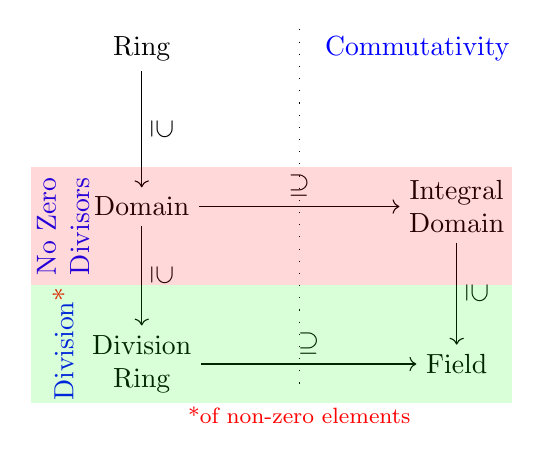
\begin{tikzpicture}
                \node (Ring) at (0,0) {Ring};
                \node (Domain) at (0,-2){Domain};
                \node[align=center] (Integral Domain) at (4,-2) {Integral\\ Domain};
                \node[align=center] (Division Ring) at (0,-4) {Division\\ Ring};
                \node (Field) at (4,-4) {Field};
                \node (Commutativity) at (3.5,0) {\textcolor{blue}{Commutativity}};
                \node[text=blue, align=center, rotate=90] (No Zero Divisors) at (-1,-2.25) {No Zero\\ Divisors};
                \node[text=blue, align=center, rotate=90] (Division*) at (-1,-3.75) {Division\textcolor{red}{*}};
                \node[text=red] (*of non-zero elements) at (2,-4.65) {{\footnotesize*of non-zero elements}};

                \draw[->] (Ring) -- (Domain) node[midway, above, sloped] {\(\supseteq\)};
                \draw[->] (Domain) -- (Integral Domain) node[midway, above, sloped] {\(\supseteq\)};
                \draw[->] (Domain) -- (Division Ring) node[midway, above, sloped] {\(\supseteq\)};
                \draw[->] (Division Ring) -- (Field) node[midway, above, sloped] {\(\supseteq\)};
                \draw[->] (Integral Domain) -- (Field) node[midway, above, sloped] {\(\supseteq\)};

                \draw[loosely dotted] (2,0.25) -- (2,-4.25);
                \fill[red, opacity=0.15] (-1.4,-1.5) rectangle (4.7,-3);
                \fill[green, opacity=0.15] (-1.4,-3) rectangle (4.7,-4.5);
                
            \end{tikzpicture}
            }
        }
        \vspace{-1pt}

        \begin{lemma}{3.3}
            Suppose \(\varphi:R\to S\) is an isomorphism. Then: (i) \(\varphi(1_R)=1_S\); (ii) \(\varphi(0_R)=0_S\); (iii) \(\varphi(-r)=-\varphi(r)\), \(\forall r\in R\); (iv) \(r\in R\) is invertible iff \(\varphi(r)\in S\) is invertible and, in that case, \((\varphi(r))^{-1}=\varphi(r^{-1})\); (v) \(r\in R\) is nilpotent iff \(\varphi(r)\) is nilpotent and, in that case, they have the same index of nilpotence.
        \end{lemma}

        \begin{proof}
            (i): Let \(s\in S\). Since \(\varphi\) is bijective, \(s=\varphi(r)\) for some \(r\in R\). Then \(\varphi(1_R)s=\varphi(1_R)\varphi(r)=\varphi(r)=s\) and similarly \(s\varphi(1_R)=s\), hence \(\varphi(1_R)=1_S\).

            (ii): \(\varphi(0_R)+1_S=\varphi(0_R)+\varphi(1_R)=\varphi(1_R)=1_S\), so \(\varphi(0_R)=0_S\).

            (iii): \(\varphi(-r)+\varphi(r)=\varphi(0_R)=0_S\), so \(\varphi(-r)=-\varphi(r)\).

            (iv): If \(r\) is invertible then \(\varphi(r^{-1})\varphi(r)=\varphi(r^{-1}r)=1_S\) and \(\varphi(r)\varphi(r^{-1})=\varphi(rr^{-1})=1_S\), so \(\varphi(r)\) is invertible with \((\varphi(r))^{-1}=\varphi(r^{-1})\). Conversely, apply this to \(\varphi^{-1}:S\to R\).

            (v): Since \((\varphi(r))^n=\varphi(r^n)\), \(r^n=0_R\) iff \((\varphi(r))^n=0_S\). Thus the least such \(n\) is the same.
        \end{proof}

        \vspace{2pt}
        {\centering\fontsize{7.8}{8.5}\selectfont\textbf{Definitions}\par}
        \vspace{2pt}

        \begin{definition}{1.4}
            \(\forall a,b\in\mathbb{Z}\), \(\gcd(a,b)=\max\{n\in\mathbb{Z}:n|a\;\&\;n|b\}\), noting \(\gcd(0,0)=0\) \& if \(\gcd(a,b)=1\) then \(a\) \& \(b\) are coprime.
        \end{definition}

        \begin{definition}{1.6}
            \(\forall a,b,n\in\mathbb{Z}\) with \(n\ge2\).
            \(a\) is \textbf{congruent to} \(b\) \textbf{modulo} \(n\) iff \(n|a-b\), written \(a\equiv b\mod n\).Then define the congruence class of \(a\) w.r.t. \(n\) as: \([a]_n=\{b\in\mathbb{Z}:b\equiv a\mod n\}=\{b\in\mathbb{Z}:n\mid(b-a)\}=\{a+kn:k\in\mathbb{Z}\}\)
            
            We thus have: 
            
            \fitdisplay{\(\mathbb{Z}_n=\{[a]_n:a\in\mathbb{Z}\}=\{[0]_n,[1]_n,\ldots,[n-1]_n\}\)}

            {\footnotesize Note: \(b\equiv a \mod n\) iff \(b=a+kn\) iff \([a]_n=\{a+nk:k\in\mathbb{Z}\}\) iff \([a]_n=[a+kn]_n\)}
        \end{definition}

        \begin{definition}{1.14}
            A \textbf{ring} is a set \(R\) with two binary operations \(+\) \& \(\times\), defined on \(R\), satisfying the following:

            (R1) \((R,+)\) is an abelian group with identity 0.

            (R2) \(\times\) is associative.

            (R3) \(\times\) distributes over \(+\) i.e.:

            \fitdisplay{\(\begin{aligned}a(b+c)&=ab+ac,\\(a+b)c&=ac+bc,\quad \forall a,b,c\in R\end{aligned}\)}

            (R4) The multiplicative identity \(1\in R\) \& \(1\ne0\)


        \end{definition}

        \begin{example}
            With \(n\ge 2\), \(M_n(R)\) is the ring of \(n\times n\) matrices, a non-commutative ring.
            {\footnotesize Note: the only two-sided ideals of \(M_n(F)\), \(F\) a field, are \(M_n(F)\) \& \(\{\mathbf{0}\}\) but this isn't a division ring hence even relaxing commutative in Pro\textsuperscript{p} 3.22 doesn't yeild the same pro\textsuperscript{p} with field \(\to\) division ring.}
        \end{example}

        \begin{example}
            For \(X\) a set \(\mathcal{P}(X)\) with
            
            \fitdisplay{\(\begin{aligned}A+B&=(A\cup B)\setminus(A\cap B),\\ AB&=A\cap B\end{aligned}\)}

            \& \(0=\varnothing\), \(-A=A\), \(A,B\in\mathcal{P}(X)\).
        \end{example}

        \begin{definition}{1.17}
            Let \(R\) be a ring \& \(S\subseteq R\). Then \(S\) is a \textbf{subring} of \(R\) if \(S\) is a ring w.r.t. the same addition \& multiplication as \(R\) \& contains the multiplicative identity of \(R\), \(1_R\).
        \end{definition}

        \begin{definition}{1.21}
            let \(R\) be a ring. The \textbf{ring of polynomials} \(R[X]=\{\sum_{i\ge0}^na_iX^i\text{ a finite sum}:a_i\in R\}\) with addition \& multiplication defined as:
            
            \(\sum_{i\ge0}^na_iX^i+\sum_{i\ge0}^mb_iX^i=\sum_{i\ge0}^{\max(n,m)}(a_i+b_i)X^i\)
            
            \&
            
            \(\big(\sum\limits_{i\ge0}^na_iX^i)(\sum\limits_{i\ge0}^mb_iX^i)=\sum\limits_{i\ge0}^{n+m}(\sum\limits_{j=0}^ia_{j}b_{i-j})X^i\)
            
            \(0=\sum_{i\ge0}0X^i\) \& \(1=1X^0+\sum_{i\ge1}0X^i\). Then the \textbf{degree} of a polynomial is the greatest \(i\in\mathbb{N}\cup\{0\}\) s.t. \(a_i\ne0\) or if no such \(i\) exist \(\deg(0)=-\infty\)

            More genearlly, we have:
            
            \fitdisplay{\(R[X_1,\ldots,X_n]=R[X_1,\ldots,X_{n-1}][X_n]\)}

            {\footnotesize \(\forall f,g\in R[X]\), \(\deg(f+g)\le\max(\deg(f),\deg(g))\)} \& \(\deg(fg)\le\deg(f)+\deg(g)\).
        \end{definition}

        \begin{definition}{1.24}
            If \(R_1\) \& \(R_2\) are rings then the \textbf{Cartesian product} \(R_1\times R_2\) with the \(+\) \& \(\times\) defined element wise is a ring.
        \end{definition}

        \begin{definition}{2.1}
            For \(a\in R\) define: for \(n\in\mathbb{Z}^+\), \(n\cdot a=\underbrace{a+a+\cdots+a}_{n\text{ times}}\); for \(n=0\), \(n\cdot a=0\cdot a=0\); \& for \(n\in\mathbb{Z}^-\), \(n\cdot a=(-n)\cdot(-a)\).
            
            The \textbf{Characteristic}, \(\text{char}(R)\), of a ring \(R\) is the least posititve integer \(n\) s.t. \(n\cdot 1=0\), or if no exist \(\text{char}(R)=0\).
            
            {\footnotesize Note: \((n+m)\cdot a=n\cdot a+m\cdot a\), \(n\cdot(a+b)=n\cdot a+n\cdot b\), \& \(n\cdot(m\cdot a)=(nm)\cdot a\), all easily verifiable.}
        \end{definition}

        \begin{definition}{2.3}
            A non-zero element \(r\in R\) is a \textbf{zero-divisor} if \(\exists s\in R\) a non-zero element s.t. \(rs=0\) or \(sr=0\).

            A ring \(R\) is a domain if, \(\forall r,s\in R\):

            \fitdisplay{\(rs=0\implies r=0 \text{ or } s=0.\)}

            i.e. a ring with no zero divisors is a domain \& vice versa.
        \end{definition}

        \begin{definition}{2.9}
            A \textbf{division ring} is a ring where every non-zero element has a right \& left inverse, i.e.: \(\forall r\in R\setminus\{0\},\exists s,t\in R\text{ s.t. }rs=1=tr\) with \(s\),\(t\) being the right \& left inverses, respectively.

            {\footnotesize Note: this immediately collapse, due to Le\textsuperscript{m} 2.11, to just there exists an inverse as \(s=t\).}
            
            An \textbf{invertible} element \(r\) is called a \textbf{unit}.
        \end{definition}

        \begin{example}
            Division rings are not all fields e.g. the quaternions \(\mathbb{H}=\{a+bi+cj+dk:a,b,c,d\in\mathbb{R}\}\) where \(i^2=j^2=k^2=-1\) \& \(ij=k\), \(jk=i\), \& \(ki=j\), this is non-commutative as \(-ij=-k=jjk=ji\) so \(ij\ne ji\) and this is a division ring as for \(z=a+bi+cj+dk\) \(z^{-1}=\frac{a-bi-cj-dk}{a^2+b^2+c^2+d^2}\), taking \(z\ne0\).
        \end{example}
       
        \begin{definition}{2.16}
            An element \(r\) of a ring \(R\) is \textbf{nilpotent} if \(\exists n\in\mathbb{Z}^+\) s.t. \(r^n=0\), and the least such \(n\) is the \textbf{index of nilpotence} of \(r\).

            An element \(r\in R\) is \textbf{idempotent} if \(r^2=r\).

            {\footnotesize Note: In any ring \(R\), \(0_R\) is nilpotent with index 1 and \(0_R\) and \(1_R\) are idempotent.}
        \end{definition}

        \begin{definition}{3.1}
            If \(R\) \& \(S\) are rings then an \textbf{isomorphism} from \(R\) to \(S\) is a bijection \(\varphi:R\to S\) s.t. \(\forall r,r'\in R\):

            \fitdisplay{\(\begin{aligned}\varphi(r+r')&=\varphi(r)+\varphi(r'),\\ \varphi(rr')&=\varphi(r)\varphi(r')\end{aligned}\)}

            If \(\varphi\) is an isomorphism from \(R\) to \(S\) then \(R\) \& \(S\) are \textbf{isomorphic}, written \(R\cong S\).
        \end{definition}

        \newpage

    \end{multicols}

\end{document}
